\begin{pa} \label{PA:11.1} In this activity we introduce the concept of a double Riemann sum. 
    \ba
    \item  Review the concept of the Riemann sum from single-variable calculus. Then, explain how we define the definite integral $\int_a^b f(x) \ dx$ of a continuous function of a single variable $x$ on an interval $[a,b]$. Include a sketch of a continuous function on an interval $[a,b]$ with appropriate labeling in order to illustrate your definition.


    \item In our upcoming study of integral calculus for multivariable functions, we will first extend the idea of the single-variable definite integral to functions of two variables over rectangular domains. To do so, we will need to understand how to partition a rectangle into subrectangles. Let $R$ be rectangular domain $R = \{(x,y) : 0 \leq x \leq 6, 2 \leq y \leq 4\}$ (we can also represent this domain with the notation $[0,6] \times [2,4]$), as pictured in Figure \ref{F:11.1.Domain}. 
    
        \begin{figure}[ht]
\begin{center}
  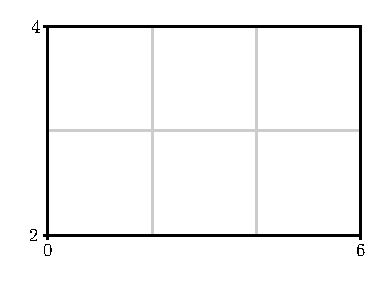
\includegraphics{figures/fig_11_1_rect_domain.eps}
\end{center}
\caption{Rectangular domain $R$ with subrectangles.}
\label{F:11.1.Domain}
\end{figure}
    
To form a partition of the full rectangular region, $R$, we will partition both intervals $[0,6]$ and $[2,4]$; in particular, we choose to partition the interval $[0,6]$ into three uniformly sized subintervals and the interval $[2,4]$ into two evenly sized subintervals as shown in Figure \ref{F:11.1.Domain}. In the following questions, we discuss how to identify the endpoints of each subinterval and the resulting subrectangles.
            \begin{enumerate}[i.]
            \item Let $0=x_0 < x_1 < x_2 < x_3=6$ be the endpoints of the subintervals of $[0,6]$ after partitioning. What is the length $\Delta x$ of each subinterval $[x_{i-1},x_i]$ for $i$ from 1 to 3?
	

    \item Explicitly identify $x_0$, $x_1$, $x_2$, and $x_3$. On Figure \ref{F:11.1.Domain} or your own version of the diagram, label these endpoints.
    	
		
	       \item Let $2=y_0 < y_1 < y_2=4$ be the endpoints of the subintervals of $[2,4]$ after partitioning. What is the length $\Delta y$ of each subinterval $[y_{j-1},y_j]$ for $j$ from 1 to 2? Identify $y_0$, $y_1$, and $y_2$ and label these endpoints on Figure \ref{F:11.1.Domain}.
	

	       \item Let $R_{ij}$ denote the subrectangle $[x_{i-1},x_i] \times [y_{j-1},y_j]$.  Appropriately label each subrectangle in your drawing of Figure \ref{F:11.1.Domain}.  How does the total number of subrectangles depend on the partitions of the intervals $[0,6]$ and $[2,4]$?
	
	
	       \item What is area $\Delta A$ of each subrectangle?

            \end{enumerate}
	\ea
\end{pa}


\begin{activitySolution}
    \ba
    \item  We approximated the area under the graph of a positive function $f$ on an interval $[a,b]$ by adding areas of rectangles. The process was to subdivide the interval $[a,b]$ into smaller subintervals, construct rectangles on each of these smaller intervals to approximate the region under the curve on that subinterval, then use the sum of the areas of these rectangles to approximate the area under the curve.

%\begin{figure}[ht]
%\begin{center}
%\resizebox{!}{2.0in}{\includegraphics{11_1_Riemann_Sum_1}}
%\end{center}
%\caption{A Riemann sum approximating the area under a curve}
%\label{F:11.1.Riemann_Sum_1}
%\end{figure}

In more detail, we started with a continuous function $f$ on a closed interval $[a,b]$. We then partitioned the interval $[a, b]$ into $n$ subintervals of equal length $\Delta x = \frac{b-a}{n}$. Let $x_0$, $x_1$, $\ldots$, $x_n$ be the endpoints of these subintervals, where $a = x_0<x_1<x_2 < \cdots < x_n = b$. We chose a point $x_i^*$ in each subinterval $[x_{i-1},x_i]$ and constructed a rectangle $R_i$ with base the interval  $[x_{i-1},x_i]$ and height $x_i^*$. The area of the rectangle $R_i$ is $f\left(x_i^*\right) \cdot \Delta x$. We then approximate the area under the curve defined by $f$ on the interval $[a,b]$ by the sum
\[\sum_{i=1}^n f\left(x_i^*\right) \cdot \Delta x.\]
%Figure \ref{F:11.1.Riemann_Sum_1} illustrates this process using 15 rectangles to approximate the area under the curve.

If we let $n$ go to infinity, we obtain the exact area under the curve and call this the definite integral of $f$ on the interval $[a,b]$:
\[\int_a^b f(x) \ dx = \lim_{n \to \infty} \sum_{i=1}^n f\left(x_i^*\right) \cdot \Delta x.\]


    \item We determine the endpoints of each subinterval and the resulting subrectangles.
            \begin{enumerate}[i.]
            \item Since these partition points are uniformly spaced, the distance between them is $\Delta x = \frac{6-0}{3} = 2$.

		\item Because $\Delta x = 2$, we have
\[x_0 = 0, \ \ \ x_1 = 2, \ \ \ x_2 = 4, \ \ \ \text{ and } \ \ \ x_3 = 6.\]
These points are labeled in the figure below. %in Figure \ref{F:11.1.Domain_s}.
%\begin{figure}[ht]
\begin{center}
\setlength{\unitlength}{1.0cm}
\begin{picture}(6.5,4.5)
\put(-0.1,-0.3){$x_0$}
\put(1.85,-0.3){$x_1$}
\put(3.85,-0.3){$x_2$}
\put(5.85,-0.3){$x_3$}
\put(-0.45,0.05){$y_0$}
\put(-0.45,1.9){$y_1$}
\put(-0.45,3.9){$y_2$}
\put(0,0){\line(1,0){6}}
\put(0,2){\line(1,0){6}}
\put(0,4){\line(1,0){6}}
\put(0,0){\line(0,1){4}}
\put(2,0){\line(0,1){4}}
\put(4,0){\line(0,1){4}}
\put(6,0){\line(0,1){4}}
\put(0.7,0.9){$R_{11}$}
\put(2.7,0.9){$R_{21}$}
\put(4.7,0.9){$R_{31}$}
\put(0.7,2.9){$R_{12}$}
\put(2.7,2.9){$R_{22}$}
\put(4.7,2.9){$R_{32}$}
\end{picture}
\end{center}
%\caption{Labeled rectangular domain $R$ with subrectangles.}
%\label{F:11.1.Domain_s}
%\end{figure}
		
	       \item Here we have $\Delta y = \frac{4-2}{2} = 1$, and so
\[y_0 = 2, \ \ \ y_1 = 3, \ \ \ \text{ and } \ \ \ y_2 = 4.\]
These points are labeled in Figure \ref{F:11.1.Domain_s}.
	
	       \item If we partition the interval $[0,6]$ into $m$ subintervals and the interval $[2,4]$ into $n$ subintervals, that will partition the rectangle $R$ into $mn$ subintervals. The subrectangles $R_{ij}$ for our particular partition are labeled in Figure \ref{F:11.1.Domain_s}.

	
	       \item The area of a rectangle is length times width, so $\Delta A = \Delta x \ \Delta y$.


            \end{enumerate}
	\ea

\end{activitySolution}

 \afterpa 